% !Mode:: "TeX:UTF-8"

\appendix
\section{\centering 设计图纸}

\subsection{系统总框图}
本智能手表系统以STM32F103C8T6为主控制器，通过I2C和USART总线连接三大外设模块，手机端通过蓝牙SPP协议与手表交互。系统完整原理图如图\ref{fig:ap_arch}所示。

\begin{figure}[h]
    \centering
    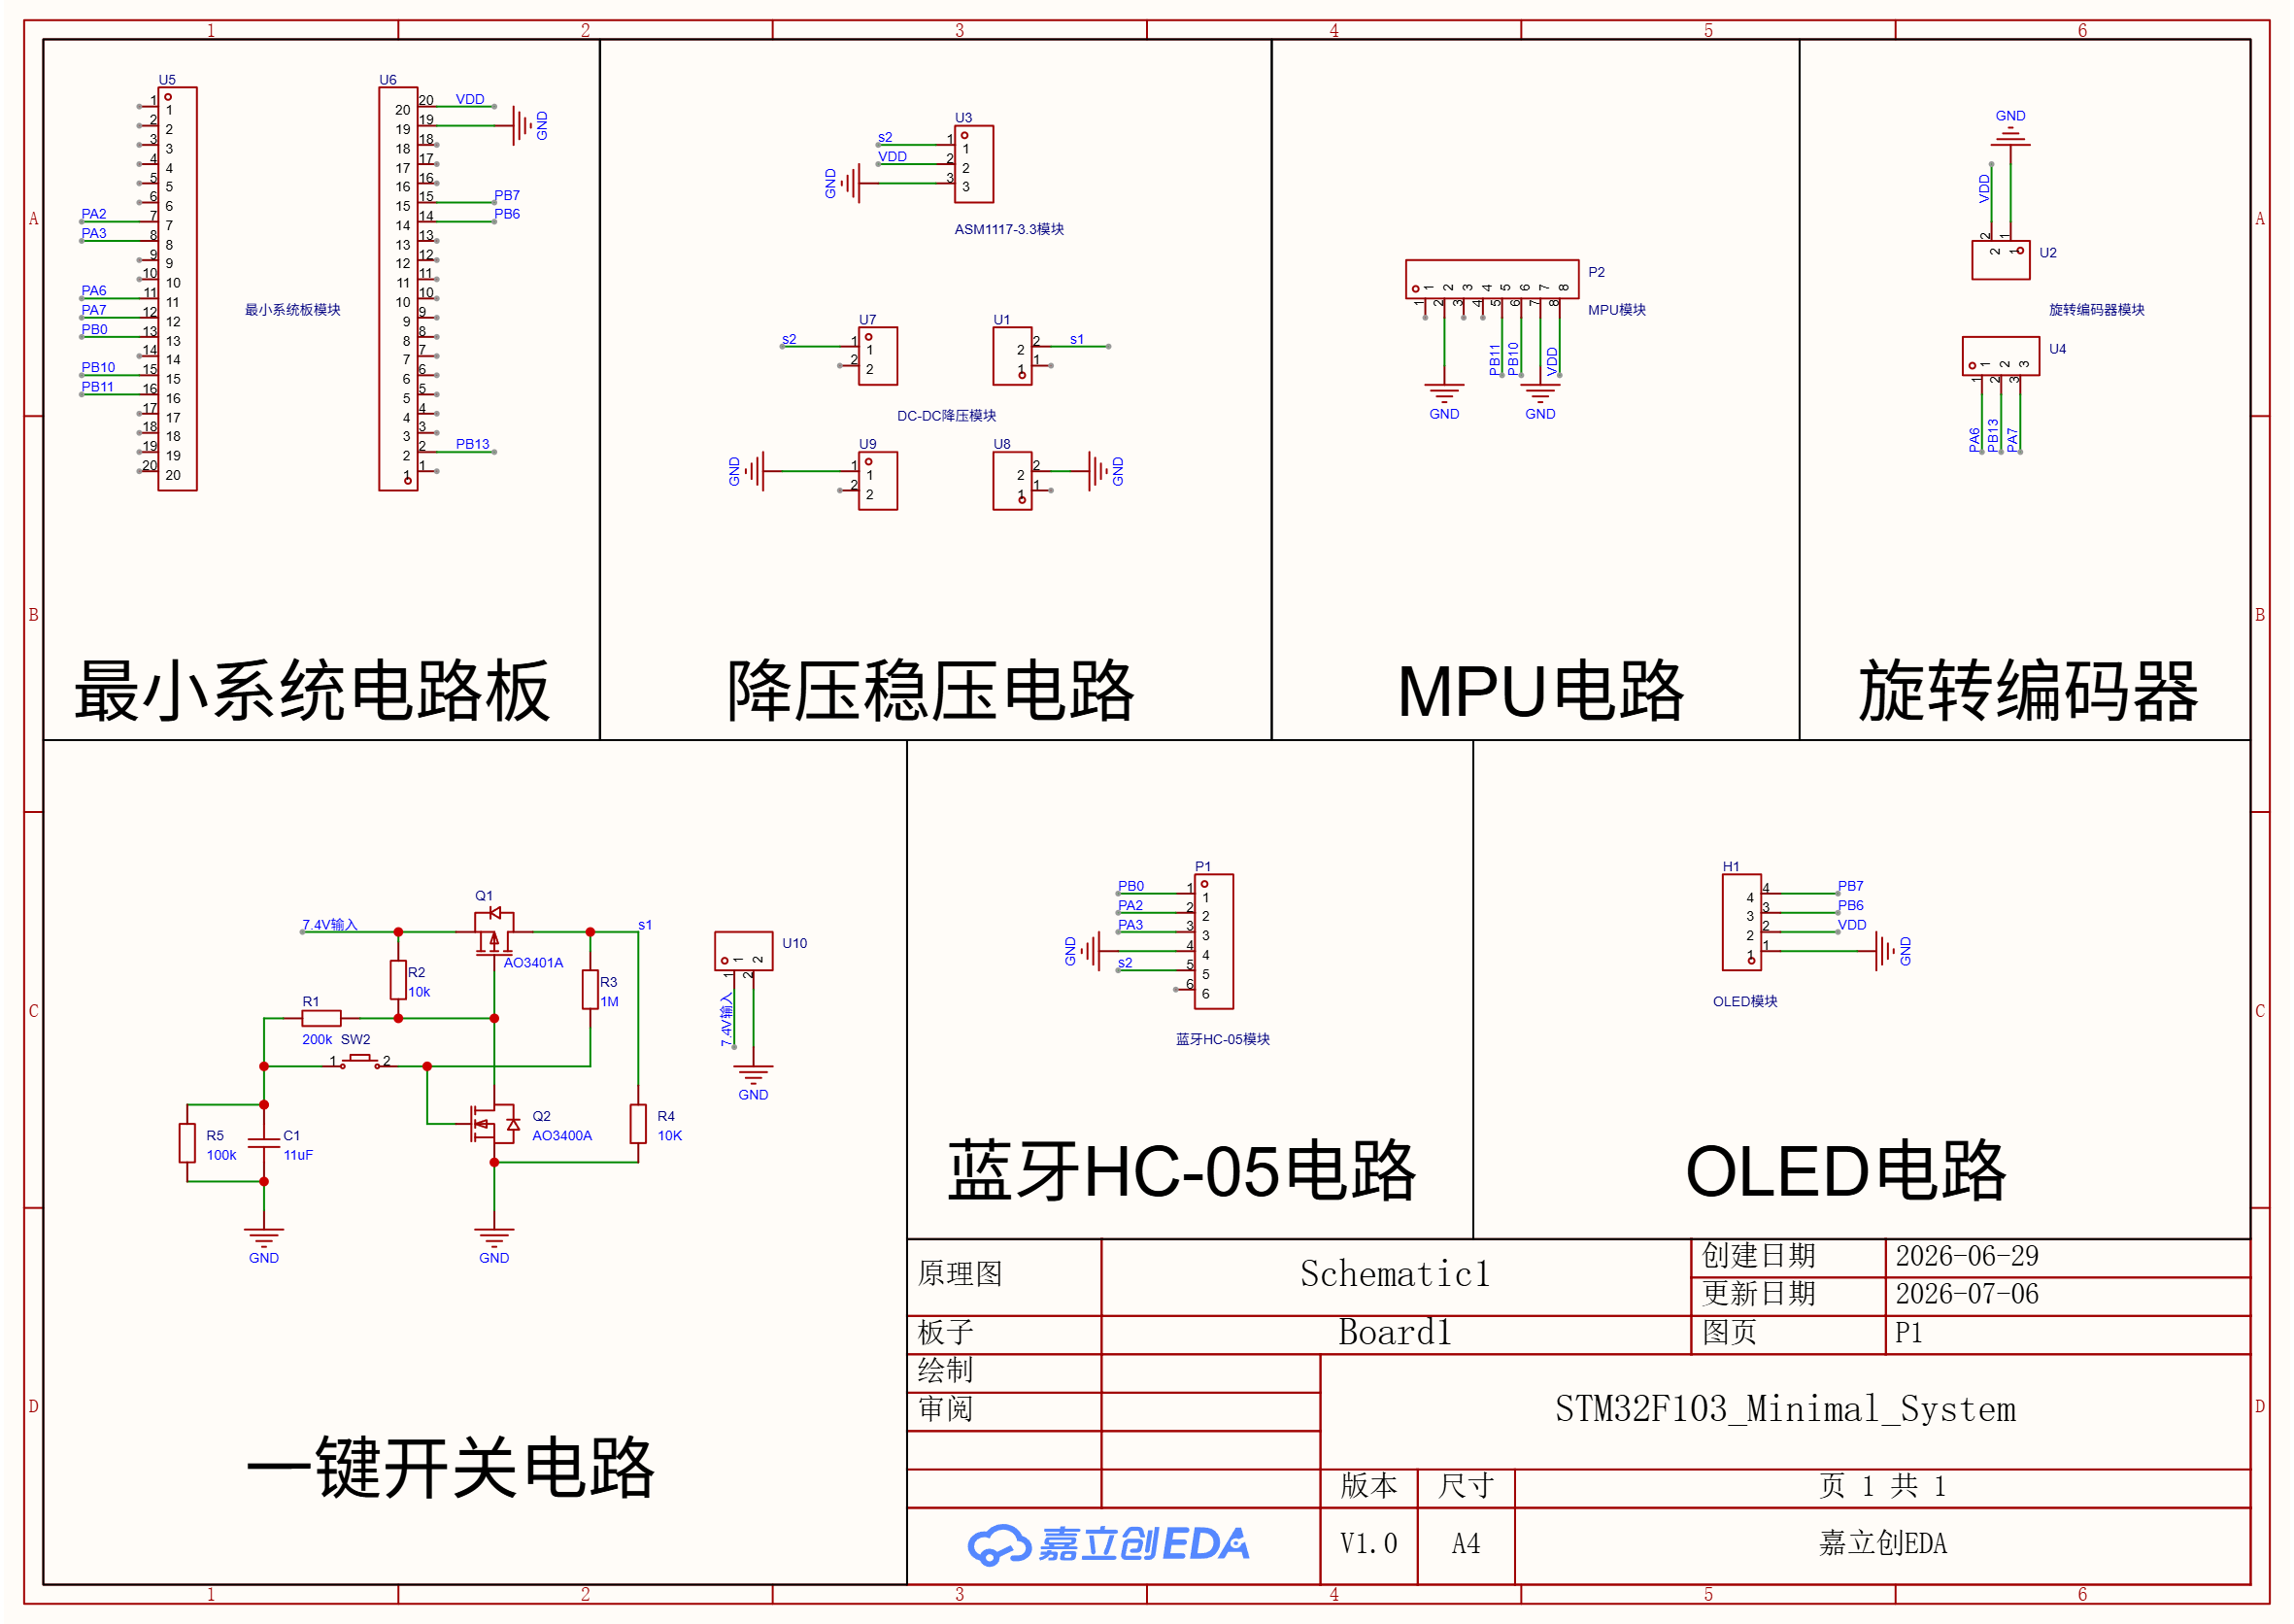
\includegraphics[width=0.95\textwidth]{figures/原理图终版.png}
    \caption{智能手表系统完整原理图（核心板 + 外设模块总线连接）}
    \label{fig:ap_arch}
\end{figure}

\FloatBarrier

\subsection{硬件引脚连接图}
各模块与STM32F103C8T6的引脚连接如表\ref{tab:ap_pinmap}所示，确保信号流向正确、电源与地分离设计。

\begin{table}[h]
    \centering
    \caption{硬件引脚连接表}
    \label{tab:ap_pinmap}
    \begin{tabular}{|l|l|l|l|}
        \hline
        \textbf{模块名称} & \textbf{模块引脚} & \textbf{STM32引脚} & \textbf{功能} \\ \hline
        SSD1306 OLED & VCC & 3.3V & 电源 \\ \hline
        SSD1306 OLED & GND & GND & 地 \\ \hline
        SSD1306 OLED & SCL & PB6 (I2C1\_SCL) & I2C时钟 \\ \hline
        SSD1306 OLED & SDA & PB7 (I2C1\_SDA) & I2C数据 \\ \hline
        MPU6050 & VCC & 3.3V & 电源 \\ \hline
        MPU6050 & GND & GND & 地 \\ \hline
        MPU6050 & SCL & PB10 (I2C2\_SCL) & I2C时钟 \\ \hline
        MPU6050 & SDA & PB11 (I2C2\_SDA) & I2C数据 \\ \hline
        HC-05蓝牙 & VCC & 5V & 电源 \\ \hline
        HC-05蓝牙 & GND & GND & 地 \\ \hline
        HC-05蓝牙 & TX & PA3 (USART2\_RX) & 模块发送→MCU接收 \\ \hline
        HC-05蓝牙 & RX & PA2 (USART2\_TX) & 模块接收←MCU发送 \\ \hline
        HC-05蓝牙 & STATE & PB0 (GPIO\_Input) & 连接状态检测 \\ \hline
        状态LED & Anode & PC13 & 运行状态指示 \\ \hline
        状态LED & Cathode & GND & 通过220$\Omega$电阻接地 \\ \hline
    \end{tabular}
\end{table}

\FloatBarrier

\subsection{软件模块调用关系}
固件软件采用分层模块化设计，主循环统一调度各功能模块。main.c作为调度中枢，调用驱动层和应用层各模块。模块间的调用关系如下：

\begin{itemize}
    \item \textbf{main.c（主循环调度器）} 直接调用以下模块的接口函数：
    \begin{itemize}
        \item oled.c — OLED显示驱动
        \item mpu6050.c — 六轴传感器驱动
        \item bluetooth.c — 蓝牙帧协议
        \item smartwatch\_ui.c — 多页面UI框架
        \item pedometer.c — 计步器算法
        \item soft\_rtc.c — 软RTC时钟
    \end{itemize}
    \item \textbf{所有功能模块} 均依赖 STM32 HAL驱动层（I2C1、I2C2、USART2、GPIO、TIM2、DMA）完成硬件交互
\end{itemize}

\FloatBarrier

\section{\centering 代码清单}

\subsection{STM32固件核心源文件}
固件源代码文件结构如表\ref{tab:ap_codefiles}所示，所有文件均位于工程Core目录下。

\begin{table}[h]
    \centering
    \caption{STM32固件源文件清单}
    \label{tab:ap_codefiles}
    \begin{tabular}{|l|l|r|l|}
        \hline
        \textbf{文件名} & \textbf{类型} & \textbf{行数} & \textbf{功能说明} \\ \hline
        main.c & 源文件 & 280 & 主循环、系统初始化、任务调度 \\ \hline
        oled.h / oled.c & 头/源文件 & 320 & SSD1306 OLED驱动与字模 \\ \hline
        mpu6050.h / mpu6050.c & 头/源文件 & 260 & MPU6050六轴传感器驱动 \\ \hline
        bluetooth.h / bluetooth.c & 头/源文件 & 220 & HC-05蓝牙帧协议实现 \\ \hline
        pedometer.h / pedometer.c & 头/源文件 & 180 & 计步器算法实现 \\ \hline
        smartwatch\_ui.h / smartwatch\_ui.c & 头/源文件 & 240 & OLED多页面UI框架 \\ \hline
        soft\_rtc.h / soft\_rtc.c & 头/源文件 & 120 & TIM2软RTC时钟实现 \\ \hline
        i2c\_drv.h / i2c\_drv.c & 头/源文件 & 80 & I2C总线恢复实现 \\ \hline
        gpio.c / usart.c / i2c.c / tim.c & 源文件 & 500 & STM32CubeMX生成的外设配置 \\ \hline
        stm32f1xx\_it.c & 源文件 & 150 & 中断服务函数（TIM2、USART2） \\ \hline
        \textbf{合计} & - & \textbf{2350} & - \\ \hline
    \end{tabular}
\end{table}

\FloatBarrier

\subsection{核心代码片段}

\subsubsection{OLED初始化代码（oled.c）}
\begin{lstlisting}[language=C, basicstyle=\ttfamily\footnotesize, numbers=left, numberstyle=\tiny, stepnumber=1, numbersep=5pt, frame=shadowbox, rulesepcolor=\color{red!20!green!20!blue!20}, keywordstyle=\color{blue}\bfseries, commentstyle=\color{codegreen}, stringstyle=\color{orange}, showstringspaces=false]
void OLED_Init(void)
{
    /* 1. 发送初始化命令序列 */
    OLED_Write_Cmd(0xAE); /* 关闭显示 */
    OLED_Write_Cmd(0x20); /* 设置内存寻址模式 */
    OLED_Write_Cmd(0x10); /* 页寻址模式 */
    OLED_Write_Cmd(0xB0); /* 设置页地址 */
    OLED_Write_Cmd(0xC8); /* COM输出扫描方向 */
    OLED_Write_Cmd(0x00); /* 设置低位列地址 */
    OLED_Write_Cmd(0x10); /* 设置高位列地址 */
    OLED_Write_Cmd(0x40); /* 设置起始行地址 */
    OLED_Write_Cmd(0x81); /* 设置对比度 */
    OLED_Write_Cmd(0xFF); /* 最大对比度 */
    OLED_Write_Cmd(0xA1); /* 段重映射 */
    OLED_Write_Cmd(0xA6); /* 正常显示模式 */
    OLED_Write_Cmd(0xA8); /* 设置多路复用率 */
    OLED_Write_Cmd(0x3F); /* 1/64 duty */
    OLED_Write_Cmd(0xA4); /* 全局显示开启 */
    OLED_Write_Cmd(0xD3); /* 设置显示偏移 */
    OLED_Write_Cmd(0x00); /* 无偏移 */
    OLED_Write_Cmd(0xD5); /* 设置时钟分频因子 */
    OLED_Write_Cmd(0xF0); /* 高频时钟 */
    OLED_Write_Cmd(0xD9); /* 设置预充电周期 */
    OLED_Write_Cmd(0x22); /* 标准预充电 */
    OLED_Write_Cmd(0xDA); /* 设置COM引脚配置 */
    OLED_Write_Cmd(0x12); /* 标准配置 */
    OLED_Write_Cmd(0xDB); /* 设置VCOMH */
    OLED_Write_Cmd(0x20); /* 0.77*VCC */
    OLED_Write_Cmd(0x8D); /* 电荷泵设置 */
    OLED_Write_Cmd(0x14); /* 启用电荷泵 */
    OLED_Write_Cmd(0xAF); /* 开启显示 */
    OLED_Clear(); /* 清屏 */
}
\end{lstlisting}

\subsubsection{MPU6050六轴数据读取代码（mpu6050.c）}
\begin{lstlisting}[language=C, basicstyle=\ttfamily\footnotesize, numbers=left, numberstyle=\tiny, stepnumber=1, numbersep=5pt, frame=shadowbox, rulesepcolor=\color{red!20!green!20!blue!20}, keywordstyle=\color{blue}\bfseries, commentstyle=\color{codegreen}, stringstyle=\color{orange}, showstringspaces=false]
void MPU6050_Read_Accel(float *ax, float *ay, float *az)
{
    uint8_t buf[6];
    int16_t raw_x, raw_y, raw_z;

    /* 从0x3B寄存器连续读取6字节加速度数据 */
    HAL_I2C_Mem_Read(&hi2c2, MPU6050_ADDR, 0x3B, 1, buf, 6, HAL_MAX_DELAY);

    /* 组合高低字节（大端格式，高字节在前） */
    raw_x = (int16_t)((buf[0] << 8) | buf[1]);
    raw_y = (int16_t)((buf[2] << 8) | buf[3]);
    raw_z = (int16_t)((buf[4] << 8) | buf[5]);

    /* 转换为物理量（加速度量程±2g，灵敏度16384 LSB/g） */
    *ax = (float)raw_x / 16384.0f * 9.8f;  /* m/s^2 */
    *ay = (float)raw_y / 16384.0f * 9.8f;
    *az = (float)raw_z / 16384.0f * 9.8f;
}

void MPU6050_Read_Gyro(float *gx, float *gy, float *gz)
{
    uint8_t buf[6];
    int16_t raw_x, raw_y, raw_z;

    /* 从0x43寄存器连续读取6字节陀螺仪数据 */
    HAL_I2C_Mem_Read(&hi2c2, MPU6050_ADDR, 0x43, 1, buf, 6, HAL_MAX_DELAY);

    raw_x = (int16_t)((buf[0] << 8) | buf[1]);
    raw_y = (int16_t)((buf[2] << 8) | buf[3]);
    raw_z = (int16_t)((buf[4] << 8) | buf[5]);

    /* 转换为物理量（陀螺仪量程±250°/s，灵敏度131 LSB/°/s） */
    *gx = (float)raw_x / 131.0f;  /* deg/s */
    *gy = (float)raw_y / 131.0f;
    *gz = (float)raw_z / 131.0f;
}
\end{lstlisting}

\subsubsection{蓝牙帧协议发送代码（bluetooth.c）}
\begin{lstlisting}[language=C, basicstyle=\ttfamily\footnotesize, numbers=left, numberstyle=\tiny, stepnumber=1, numbersep=5pt, frame=shadowbox, rulesepcolor=\color{red!20!green!20!blue!20}, keywordstyle=\color{blue}\bfseries, commentstyle=\color{codegreen}, stringstyle=\color{orange}, showstringspaces=false]
void Bluetooth_Send_Frame(uint8_t cmd, uint8_t *data, uint16_t len)
{
    uint8_t frame[256];
    uint8_t checksum = 0;
    uint16_t idx = 0;
    uint16_t i;

    /* 1. 组装帧格式：STX(0xAA) + CMD + DATA + CHK(XOR) + ETX(0x55) */
    frame[idx++] = 0xAA;          /* 帧头 */
    frame[idx++] = cmd;           /* 命令字节 */

    /* 2. 填充数据载荷 */
    for (i = 0; i < len; i++)
    {
        frame[idx++] = data[i];
    }

    /* 3. 计算XOR校验（对CMD和DATA所有字节做异或） */
    checksum = cmd;
    for (i = 0; i < len; i++)
    {
        checksum ^= data[i];
    }
    frame[idx++] = checksum;     /* 校验字节 */
    frame[idx++] = 0x55;         /* 帧尾 */

    /* 4. 通过USART2发送完整帧（阻塞方式） */
    HAL_UART_Transmit(&huart2, frame, idx, HAL_MAX_DELAY);
}
\end{lstlisting}

\subsubsection{计步器算法核心代码（pedometer.c）}
\begin{lstlisting}[language=C, basicstyle=\ttfamily\footnotesize, numbers=left, numberstyle=\tiny, stepnumber=1, numbersep=5pt, frame=shadowbox, rulesepcolor=\color{red!20!green!20!blue!20}, keywordstyle=\color{blue}\bfseries, commentstyle=\color{codegreen}, stringstyle=\color{orange}, showstringspaces=false]
static float filtered_mag = 1.0f;      /* 低通滤波输出 */
static float mag_max = 1.3f;           /* 动态最大值 */
static float mag_min = 0.7f;           /* 动态最小值 */
static uint32_t last_step_tick = 0;    /* 上一步时间戳 */
static uint32_t step_count = 0;        /* 总步数 */

uint8_t Pedometer_Update(float ax, float ay, float az)
{
    /* 1. 计算加速度向量幅值（单位: g） */
    float mag = sqrtf(ax * ax + ay * ay + az * az) / 9.8f;

    /* 2. 一阶低通滤波（指数加权平均，α=0.7） */
    filtered_mag = 0.7f * filtered_mag + 0.3f * mag;

    /* 3. 更新滑动窗口内的最大最小值（动态阈值） */
    if (filtered_mag > mag_max) mag_max = filtered_mag;
    if (filtered_mag < mag_min) mag_min = filtered_mag;

    /* 4. 计算当前阈值（中点+偏移量） */
    float threshold = (mag_max + mag_min) * 0.5f + 0.05f;

    /* 5. 峰值检测：从低于阈值上升到高于阈值时标记为一步 */
    static uint8_t below_threshold = 1;
    uint32_t now = HAL_GetTick();
    uint8_t new_step = 0;

    if (filtered_mag < threshold)
    {
        below_threshold = 1;
    }
    else if (below_threshold && (now - last_step_tick) > 200)
    {
        /* 上升沿 + 200ms最小步间间隔 = 确认一步 */
        step_count++;
        last_step_tick = now;
        below_threshold = 0;
        new_step = 1;
    }

    /* 6. 定期重置动态阈值窗口（约每4秒） */
    static uint32_t window_reset = 0;
    if ((now - window_reset) > 4000)
    {
        mag_max = filtered_mag + 0.1f;
        mag_min = filtered_mag - 0.1f;
        window_reset = now;
    }

    return new_step;
}
\end{lstlisting}

\subsubsection{软RTC中断代码（soft\_rtc.c）}
\begin{lstlisting}[language=C, basicstyle=\ttfamily\footnotesize, numbers=left, numberstyle=\tiny, stepnumber=1, numbersep=5pt, frame=shadowbox, rulesepcolor=\color{red!20!green!20!blue!20}, keywordstyle=\color{blue}\bfseries, commentstyle=\color{codegreen}, stringstyle=\color{orange}, showstringspaces=false]
static uint8_t hour = 0, minute = 0, second = 0;
static uint8_t day = 1, month = 1;
static uint16_t year = 2025;

/* TIM2 1Hz中断服务回调（在stm32f1xx_it.c中调用） */
void Soft_RTC_Handler(void)
{
    second++;
    if (second >= 60)
    {
        second = 0;
        minute++;
        if (minute >= 60)
        {
            minute = 0;
            hour++;
            if (hour >= 24)
            {
                hour = 0;
                day++;
                /* 简化的月份天数处理（暂不考虑闰年2月） */
                uint8_t days_in_month[] = {31,28,31,30,31,30,31,31,30,31,30,31};
                if (day > days_in_month[month - 1])
                {
                    day = 1;
                    month++;
                    if (month > 12)
                    {
                        month = 1;
                        year++;
                    }
                }
            }
        }
    }
}

/* 蓝牙时间同步命令(0x02)处理：更新RTC */
void Soft_RTC_Set_Time(uint8_t h, uint8_t m, uint8_t s)
{
    if (h < 24) hour = h;
    if (m < 60) minute = m;
    if (s < 60) second = s;
}
\end{lstlisting}

\subsubsection{Android端蓝牙协议解析代码（BtProtocol.kt）}
\begin{lstlisting}[language=Kotlin, basicstyle=\ttfamily\footnotesize, numbers=left, numberstyle=\tiny, stepnumber=1, numbersep=5pt, frame=shadowbox, rulesepcolor=\color{red!20!green!20!blue!20}, keywordstyle=\color{blue}\bfseries, commentstyle=\color{codegreen}, stringstyle=\color{orange}, showstringspaces=false]
object BtProtocol {
    const val STX = 0xAA.toByte()  /* 帧头 */
    const val ETX = 0x55.toByte()  /* 帧尾 */
    const val CMD_SENSOR = 0x01.toByte()  /* 传感器数据 */
    const val CMD_TIME = 0x02.toByte()    /* 时间同步 */
    const val CMD_STEP = 0x03.toByte()    /* 计步数据 */

    /* 解析手表上报的传感器数据帧（24字节：6个float） */
    fun parseSensorData(data: ByteArray): FloatArray {
        val values = FloatArray(6)
        /* 小端格式：每个float占4字节 */
        val buffer = ByteBuffer.wrap(data).order(ByteOrder.LITTLE_ENDIAN)
        for (i in 0 until 6) {
            values[i] = buffer.float
        }
        /* values: ax, ay, az(加速度m/s^2), gx, gy, gz(陀螺仪deg/s) */
        return values
    }

    /* 组装时间同步命令下发给手表 */
    fun buildTimeSyncFrame(hour: Int, minute: Int, second: Int): ByteArray {
        val frame = ByteArray(6)
        frame[0] = STX
        frame[1] = CMD_TIME
        frame[2] = hour.toByte()
        frame[3] = minute.toByte()
        frame[4] = second.toByte()
        /* XOR校验 */
        frame[5] = (CMD_TIME.toInt() xor hour xor minute xor second).toByte()
        /* 注意：实际帧长度还需追加ETX */
        return frame + byteArrayOf(ETX)
    }
}
\end{lstlisting}

\section{\centering 参考文献}

\addcontentsline{toc}{section}{参考文献}

\begin{thebibliography}{99}

\bibitem{ref1} 刘火良，杨森. \textit{STM32库开发实战指南：基于野火STM32全系列开发板}. 机械工业出版社, 2020.

\bibitem{ref2} STMicroelectronics. \textit{STM32F103xC, STM32F103xD, STM32F103xE Reference Manual} (RM0008). Rev 21, 2023.

\bibitem{ref3} STMicroelectronics. \textit{PM0056 Programming Manual: STM32F10xxx Cortex-M3 Programming}. Rev 5, 2020.

\bibitem{ref4} Solomon Systech. \textit{SSD1306 128x64 Dot Matrix OLED/PLED Segment/Common Driver with Controller Data Sheet}. Rev 1.1, 2008.

\bibitem{ref5} TDK InvenSense. \textit{MPU-6000 and MPU-6050 Product Specification Register Map and Descriptions}. Rev 4.2, 2013.

\bibitem{ref6} HC-05 Bluetooth Module. \textit{HC-05 Product Data Sheet}. Guangzhou HC Intelligent Technology Co., Ltd.

\bibitem{ref7} Carmine Noviello. \textit{Mastering STM32} (2nd ed.). Leanpub, 2022.

\bibitem{ref8} Joseph Yiu. \textit{The Definitive Guide to ARM Cortex-M3 and Cortex-M4 Processors} (3rd ed.). Newnes, 2013.

\bibitem{ref9} 王忠飞，严冬. \textit{嵌入式系统原理及应用——基于ARM Cortex-M3内核的STM32微控制器}. 清华大学出版社, 2019.

\bibitem{ref10} Lars Bengtsson. \textit{Step Counter Using Accelerometer Data}. Technical Report, University of Gothenburg, 2019.

\bibitem{ref11} Philip Alpay. \textit{Programming Android with Kotlin: Achieving Structured Concurrency with Coroutines}. O'Reilly Media, 2021.

\bibitem{ref12} Google. \textit{Android Developers: Bluetooth Overview}. https://developer.android.com/guide/topics/connectivity/bluetooth, 2024.

\end{thebibliography}